%-------------------------------------------------------------------------------
% seq24_menu
%-------------------------------------------------------------------------------
%
% \file        seq24_menu.tex
% \library     Documents
% \author      Chris Ahlstrom
% \date        2015-08-31
% \update      2015-09-01
% \version     $Revision$
% \license     $XPC_GPL_LICENSE$
%
%     Provides the Menu section of seq24-user-manual.tex.
%
%-------------------------------------------------------------------------------

\section{Menu}
\label{sec:seq24_menu}

   The \textsl{Sequencer24} menu, as seen at the top of
   \figureref{fig:seq24_main_screen},
   is fairly simple, but it is important to understand the
   structure of the menu entries.

\subsection{Menu / File}
\label{subsec:seq24_menu_file}

   The \textbf{File} menu is used to save and load standard 
   MIDI files.  It should be able to handle any 
   Format 1 standard files that any other sequencer 
   is capable of exporting.  

   The \textsl{Sequencer24}
   menu entry contains the sub-items shown in
   \figureref{fig:seq24_menu_file_items}.
   The next few sub-sections discuss the sub-items in the 
   \textsl{File} sub-menu.

\begin{figure}[H]
   \centering 
   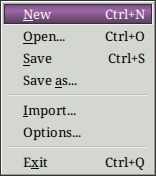
\includegraphics[scale=0.75]{menu/menu_file.png}
   \caption{Sequencer24 File Menu Items}
   \label{fig:seq24_menu_file_items}
\end{figure}

   \begin{enumber}
      \item \textbf{New}
      \item \textbf{Open...}
      \item \textbf{Save}
      \item \textbf{Save As...}
      \item \textbf{Import...}
      \item \textbf{Options...}
      \item \textbf{Exit}
   \end{enumber}

\subsection{Menu / File / New}
\label{subsec:menu_file_new}

   The \textbf{New} menu entry clears out any current song and patterns,
   allowing one to create news ones from scratch.
   If unsaved changes are pending, the user will be prompted to save the
   changes.
   Currently, the detection of situations requiring a save (or not requiring
   a save) needs a bit of work.

\subsubsection{Menu / File / Open}
\label{subsubsec:seq24_menu_file_open}

   The \textbf{Open} menu entry opens a song that had been saved previously.
   It opens up a standard GTK+ file dialog.

\begin{figure}[H]
   \centering 
   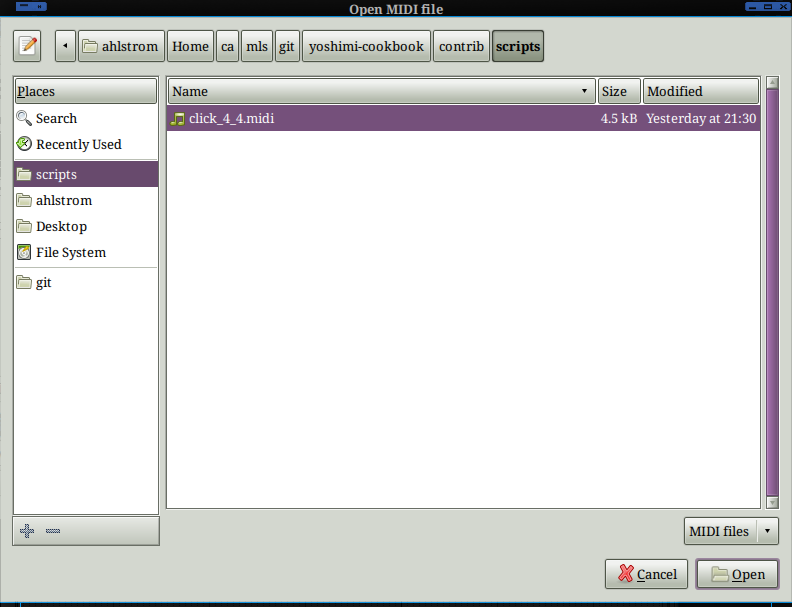
\includegraphics[scale=0.65]{menu/menu_file_open.png}
   \caption{File Open}
   \label{fig:seq24_menu_file_open}
\end{figure}

   If unsaved changes are pending, the user will be prompted to save the
   changes.

\subsubsection{Menu / File / Save and Save As}
\label{subsubsec:menu_file_open_save_as}

   The \textbf{Save} menu entry saves the song under its current name.
   If there is no current name, then
   it opens up a standard GTK+ file dialog.

   The \textbf{Save As} menu entry saves a song under a different name.
   It opens up the following standard GTK+ file dialog.

\begin{figure}[H]
   \centering 
   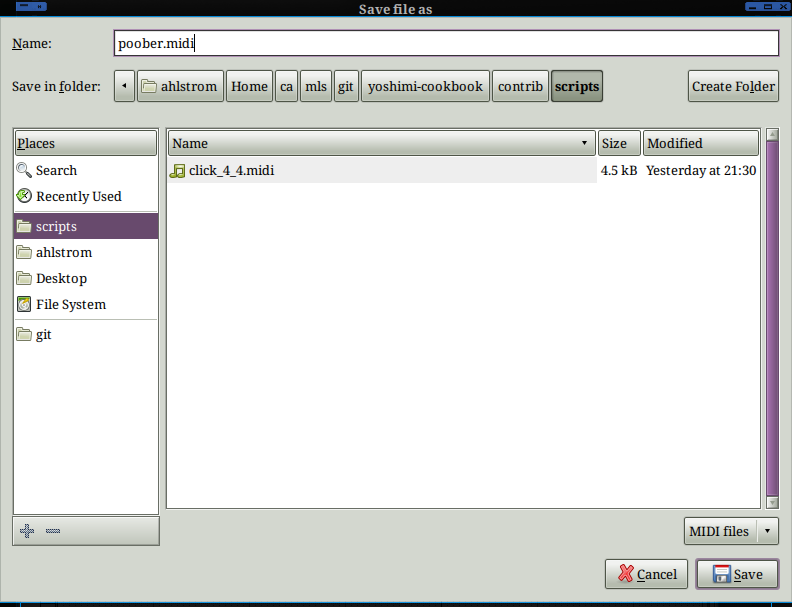
\includegraphics[scale=0.65]{menu/menu_file_save_as.png}
   \caption{File Save As}
   \label{fig:seq24_menu_file_save_as}
\end{figure}

   To save a new file, or to save the current existing file to a new name,
   enter the name in the name field, \textsl{without an extension}.
   \textsl{Sequencer24} will append a \texttt{.midi} extension to the filename.

   The file will be save in a format the the Linux \textsl{file} command
   will tag as something like:

   \begin{verbatim}
      myfile.midi: Standard MIDI data (format 1) using 16 tracks at 1/192
   \end{verbatim}

   \index{todo!solve seq24 format}
   It looks like a simple MIDI file, and yet, if one re-opens it in
   \textsl{Sequencer24}, one sees that all of the labelling, pattern information,
   and song layout has been preserved in this file.
   Even the pattern subsections, as discussed in
   \sectionref{subsubsec:seq24_song_editor_arrangement_panel_roll},
   have been saved.
   (But the L and R marker positions are not saved.)

   Compare the sizes of the original project MIDI file,
   \texttt{contrib/b4uacuse.mid}, and the output MIDI file after
   \textsl{Sequencer24} saved the patterns and the song layout we created,
   \texttt{contrib/b4uacuse-seq24.midi}.  The latter is a lot
   bigger.  

\subsubsection{Menu / File / Import}
\label{subsubsec:seq24_menu_file_import}

   The \textbf{Import} menu entry allows one to import a MIDI file
   into a pattern.

\begin{figure}[H]
   \centering 
   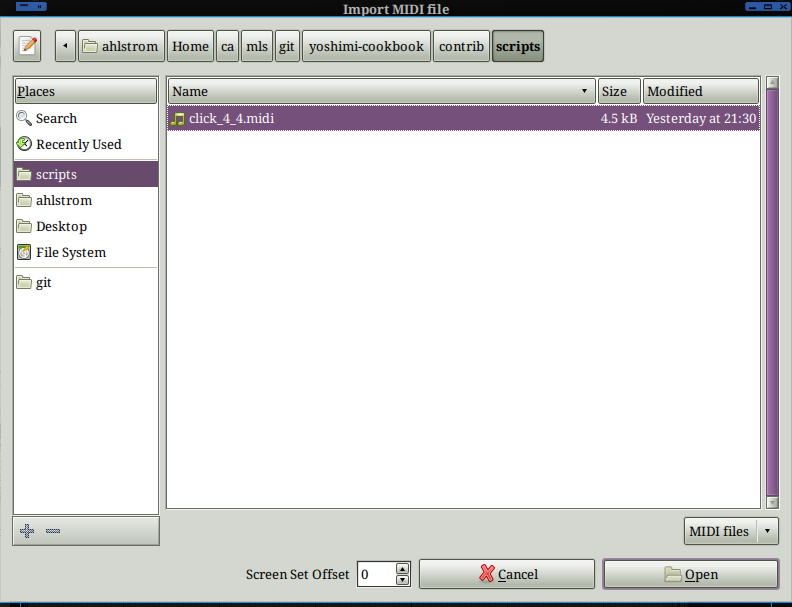
\includegraphics[scale=0.65]{menu/menu_file_import.png}
   \caption{File Import}
   \label{fig:seq24_menu_file_import}
\end{figure}

   When imported, each track, whether a music track or an information track,
   is entered into its own loop/pattern box.  The import operation can
   handle reasonably complex files, as shown in the following diagram, which
   shows an import of the \texttt{contrib/b4uacuse.mid} file, which contains
   a transcription of an Eric Clapton tune that we'd made over 20 
   years ago and had uploaded to the \textsl{GEnie} network service.

\begin{figure}[H]
   \centering 
   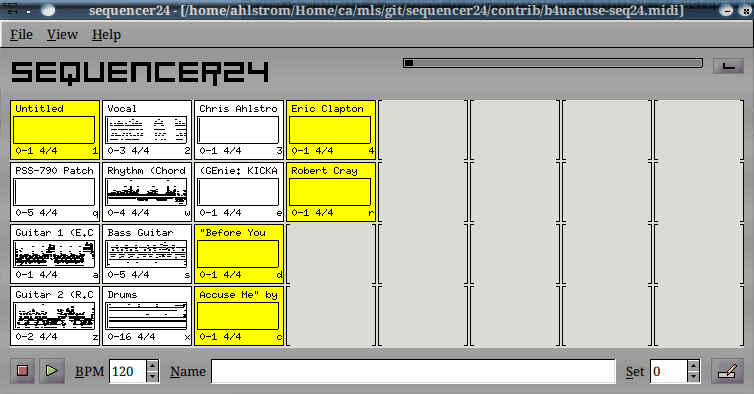
\includegraphics[scale=0.90]{menu/imported_midi_song.png}
   \caption{Imported MIDI Song}
   \label{fig:seq24_imported_midi_song}
\end{figure}

   Unfortunately, this song was created before the days of General MIDI.
   It is scored for the Yamaha PSS-790 consumer-level synthesizer.
   One can use our MIDI-conversion project (see reference \cite{midicvt}) 
   to convert it to General MIDI format, including General MIDI drums.

\subsubsection{Menu / File / Options}
\label{subsubsec:seq24_menu_file_options}

   The \textbf{Options} menu item provides a number of settings in one
   tabbed dialog, shown in the figure below.
   This dialog allows one to select which sequence gets the MIDI
   clock, which incoming MIDI events control the sequencer, what keys are
   mapped to functions, how the mouse works, and some JACK parameters.

\paragraph{Menu / File / Options / MIDI Clock}
\label{paragraph:seq24_menu_file_options_midi_clock}

   The \textbf{MIDI Clock} tab provides a way to send the MIDI clock to one
   or more of the \textsl{Sequencer24} output busses.
   It is used to configure to what busses the MIDI clock gets dumped.

\begin{figure}[H]
   \centering 
   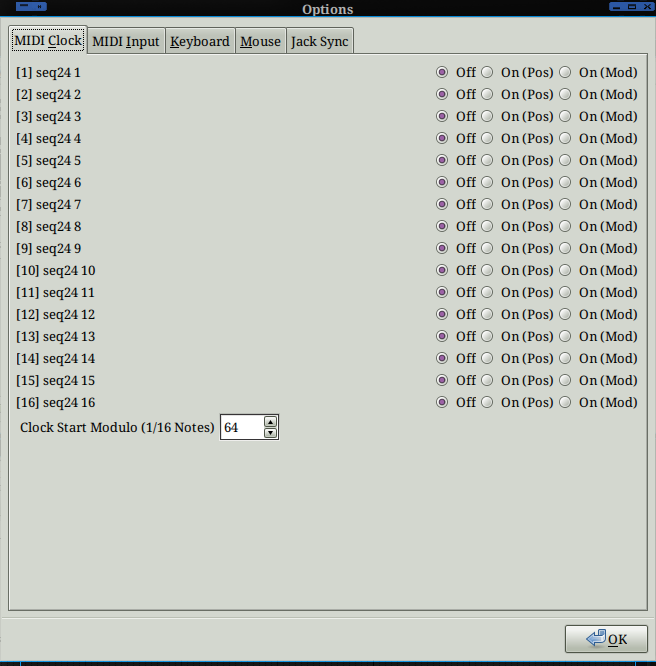
\includegraphics[scale=0.75]{menu/menu_file_options_midi_clock.png}
   \caption{File / Options / MIDI Clock}
   \label{fig:seq24_menu_file_options_midi_clock}
\end{figure}

   The following elements are present in this dialog:

   \begin{enumber}
      \item \textbf{Buss Name}
      \item \textbf{Off}
      \item \textbf{On (Pos)}
      \item \textbf{On (Mod)}
      \item \textbf{Clock Start Modulo}
   \end{enumber}

   \setcounter{ItemCounter}{0}      % Reset the ItemCounter for this list.

   \itempar{Buss Name}{midi clock!buss name}
   These labels indicate the output busses of \textsl{Sequencer24}.
   They range from \textbf{[1] seq24 1}
   to \textbf{[16] seq24 16}.

   \itempar{Off}{midi clock!off}
   This setting disables the MIDI clock for the given output buss.

   \itempar{On (Pos)}{midi clock!on (pos)}
   The MIDI clock will be sent to this buss.
   MIDI Song Position and MIDI Continue will be sent if playback is starting
   at greater than tick 0 in Song mode.  Otherwise, MIDI Start will be sent.

   \itempar{On (Mod)}{midi clock!on (mod)}
   The MIDI clock will be sent to this buss.
   MIDI Start will be sent and clocking will begin
   once the Song Position has reached the start modulo of the specified size
   (see the next item's description).
   This setting is used for gear that does not respond to Song Position.

   \itempar{Clock Start Modulo}{midi clock!clock start modulo}
   Clock Start Modulo (1/16 Notes).
   This value starts at 1 and ranges on upward to 16384.
   It  defaults to 64.
   It is used by the \textbf{On (Mod)} setting discussed above.
   It is the \texttt{[midi-clock-mod-ticks]} option in the \textsl{Sequencer24}
   "rc" file as described in
   \sectionref{subsec:seq24_rc_file_other_midi}.


\paragraph{Menu / File / Options / MIDI Input}
\label{paragraph:seq24_menu_file_options_midi_input}

   The only item in the \textbf{MIDI Input} tab is the single MIDI input
   buss provided by \textsl{Sequencer24}:  \textbf{[0] seq24 0}.

\begin{figure}[H]
   \centering 
   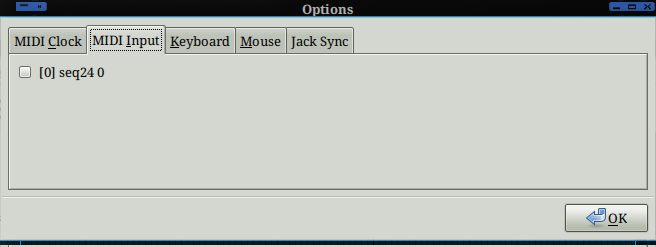
\includegraphics[scale=0.75]{menu/menu_file_options_midi_input_condensed.png}
   \caption{File / Options / MIDI Input (Condensed View)}
   \label{fig:seq24_menu_file_options_midi_input}
\end{figure}

   This item, if checked allows \textsl{Sequencer24} to be used to record MIDI
   information from another source, or pass it through to the output busses
   that are configured
   to allow pass-through
   (in the Pattern Editor, as discussed in 
   \sectionref{subsec:seq24_pattern_editor_bottom}.)

\paragraph{Menu / File / Options / Keyboard }
\label{paragraph:seq24_menu_file_options_keyboard}

   \textsl{Sequencer24}, as befits a good application, allows extensive use of
   keyboard shortcuts to make operations go faster than when using a mouse.
   The \textbf{Keyboard} tab allows for the configuration of these keyboard
   shortcuts.

\begin{figure}[H]
   \centering 
   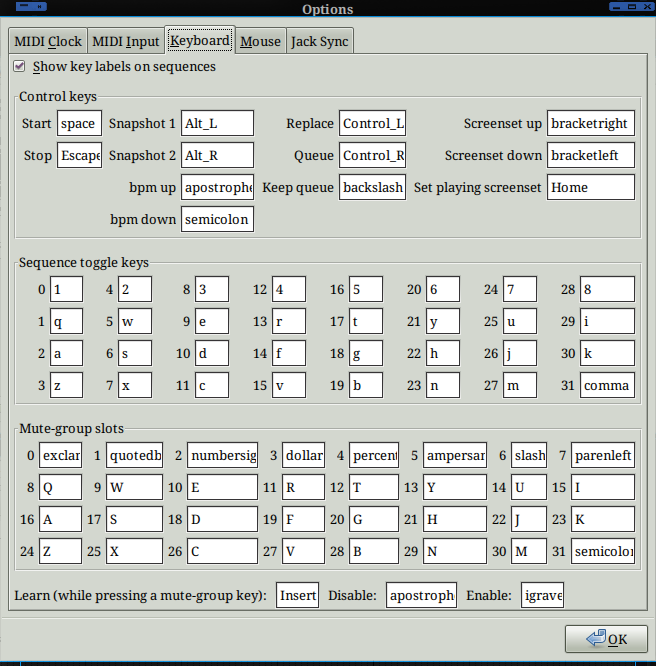
\includegraphics[scale=0.75]{menu/menu_file_options_keyboard.png}
   \caption{File / Options / Keyboard}
   \label{fig:seq24_menu_file_options_keyboard}
\end{figure}

   We won't attempt to cover every user-interface item in this busy
   dialog, just the categories.

   \begin{enumber}
      \item \textbf{Show key labels on sequences}
      \item \textbf{Control keys}
      \item \textbf{Sequence toggle keys}
      \item \textbf{Mute-group slots}
      \item \textbf{Learn}
      \item \textbf{Disable}
      \item \textbf{Enable}
   \end{enumber}

   \setcounter{ItemCounter}{0}      % Reset the ItemCounter for this list.

   \itempar{Show key labels on sequence}{keyboard!show labels}
   This item, if enabled, shows the key labels in the lower-right corner of
   each loop/pattern in the Patterns window.

   \itempar{Control keys}{keyboard!control keys}
   This block of fields provides shortcut keys for many operations of
   \textsl{Sequencer24}.

   \begin{enumber}
      \item \textbf{Start}.
         Key: \index{keys!space} \textbf{space}.
      \item \textbf{Stop}.
         Key: \index{keys!esc} \textbf{Escape}.
      \item \textbf{Snapshot 1}.
         Key: \index{keys!alt-l} \textbf{Alt\_L}.
      \item \textbf{Snapshot 2}.
         Key: \index{keys!alt-r} \textbf{Alt\_R}.
      \item \textbf{bpm up}.
         Key: \index{keys!apostrophe} \textbf{apostrophe}.
      \item \textbf{bpm down}.
         Key: \index{keys!semicolon} \textbf{semicolon}.
      \item \textbf{Replace}.
         Key: \index{keys!ctrl-l} \textbf{Control\_L}.
      \item \textbf{Queue}.
         Key: \index{keys!ctrl-r} \textbf{Control\_R}.
      \item \textbf{Keep queue}.
         Key: \index{keys!backslash} \textbf{backslash}.
      \item \textbf{Screenset down}.
         Key: \index{keys![} \textbf{bracketleft}.
      \item \textbf{Screenset up}.
         Key: \index{keys!]} \textbf{bracketright}.
      \item \textbf{Set playing screenset}.
         Key: \index{keys!home} \textbf{Home}.
   \end{enumber}

   Note that some of the keys have positional mnemonic value.  For example,
   for BPM control, the semicolon is at the left (down), and the apostrophe
   is at the right (up).

   Also note that the keys definable in this tab are only a subset of the
   various keys that can be used, especially keys used with the
   \texttt{Ctrl} key.

   TODO:  \index{todo!snapshot definition}
   One thing we need to figure out is just what this "snapshot"
   feature provides.
   \index{todo!keep queue}
   Another thing is the "queue" and "keep queue" features.

   \itempar{Sequence toggle keys}{keyboard!sequence toggle keys}
   Each of these keys toggles the playing/muting of one of the 32
   loop/pattern boxes.  These keys are layed out logically on the keyboard,
   and can also be shown in each loop/pattern box.  No need to list them all
   here!

   \itempar{Mute-group slots}{keyboard!mute-group slots}
   Each of these keys operates on the mute-grouping of one of the 32
   loop/pattern boxes.  These keys are layed out logically on the keyboard,
   and can also be shown in each loop/pattern box.  No need to list them all
   here!

   TODO: \index{todo!mute-group}
   One thing we need to discover is just what this mute-grouping
   means functionally.

   \itempar{Learn}{keyboard!learn}
   Learn (while pressing a mute-group key).
   This items sets the key used to initiate a learn mode.
   It is the \textbf{Insert} key by default.

   \itempar{Disable}{keyboard!disable}
   TODO: \index{todo!keyboard disable} What gets disabled?
   \index{keys!apostrophe}
   It is the \textbf{apostrophe} key by default.

   \itempar{Enable}{keyboard!enable}
   TODO: What gets enabled?
   \index{keys!igrave}
   It is the \textbf{igrave} (back-tick) key by default.

   There is much to learn about this learn/enable/disable triad!

\paragraph{Menu / File / Options / Mouse }
\label{paragraph:seq24_menu_file_options_mouse}

   This item selects the mouse-interaction method.

\begin{figure}[H]
   \centering 
   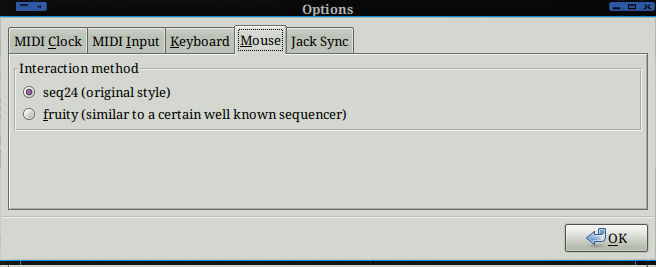
\includegraphics[scale=0.75]{menu/menu_file_options_mouse_condensed.png}
   \caption{File / Options / Mouse (Condensed View)}
   \label{fig:seq24_menu_file_options_mouse}
\end{figure}

   The default method is \textbf{seq24 (original style)}.
   The alternate method is \textbf{fruity (similar to a certain well known
   sequencer)}.

   The alternate method is presumably that of the \textsl{Fruity Loops}
   (now \textsl{FL Studio}) sequencer.  The fruity mode seems to involve the
   following (based on scanning the source code):
   
   \begin{itemize}
      \item \textbf{Left-click left side}.
         Begin a grow/shrink operation for the left side.
      \item \textbf{Left-click right side}.
         Begin a grow/shrink operation for the right side.
      \item \textbf{Left-click middle}.
         Move the object.
      \item \textbf{Left-click}.
         Add an event if nothing selected.
      \item \textbf{Middle-click}.
         Split the note?
   \end{itemize}

\paragraph{Menu / File / Options / Jack Sync }
\label{paragraph:seq24_menu_file_options_jack_sync}

   This tab sets up options for JACK synchronization.

\begin{figure}[H]
   \centering 
   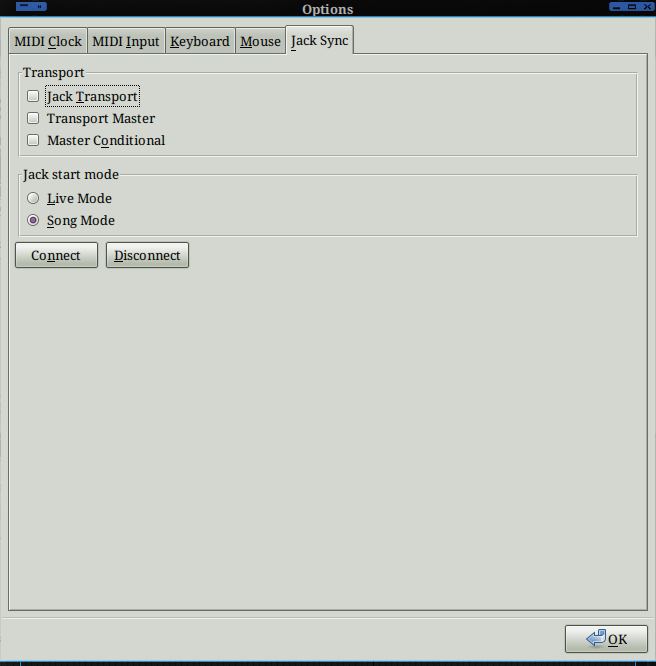
\includegraphics[scale=0.75]{menu/menu_file_options_jack_sync.png}
   \caption{File / Options / Jack Sync}
   \label{fig:seq24_menu_file_options_jack_sync}
\end{figure}

   \begin{enumber}
      \item \textbf{Transport}
      \item \textbf{Jack start mode}
      \item \textbf{Connect}
      \item \textbf{Disconnect}
   \end{enumber}

   \setcounter{ItemCounter}{0}      % Reset the ItemCounter for this list.

   \itempar{Transport}{jack sync!transport}
   This items collects the following settings:

   \begin{itemize}
      \item \textbf{Jack Transport}.
         \index{JACK!transport}
         Enables synchronization with JACK Transport.
      \item \textbf{Transport Master}.
         \index{JACK!transport master}
         \textsl{Sequencer24} will attempt to serve as the JACK Master.
      \item \textbf{Master Conditional}.
         \index{JACK!master conditional}
         \textsl{Sequencer24} will fail to serve as the JACK Master if there is
         already a Master set.
   \end{itemize}

   \itempar{Transport}{jack sync!transport}
   This items collects the following settings:

   \begin{itemize}
      \item \textbf{Live Mode}.
         \index{JACK!live mode}
         Playback will be in live mode.  Use this option to allow muting and
         unmuting of patterns.
      \item \textbf{Song Mode}.
         \index{JACK!song mode}
         Playback will use only the Song Editor's data.
   \end{itemize}

   \itempar{Connect}{jack sync!connect}
   Connect to JACK Sync.

   \itempar{Disconnect}{jack sync!disconnect}
   Disconnect from JACK Sync.

\subsection{Menu / View}
\label{subsec:seq24_menu_view}

   This menu item has only one entry, \textbf{Song Editor}, 
   which is already covered by a button at the bottom of the Patterns
   window.  Selecting this item bring up the Song Editor window.
   See \figureref{fig:song_editor_window}

\subsection{Menu / Help About...}
\label{subsec:seq24_menu_about}

   This menu entry shows the "About" dialog.

\begin{figure}[H]
   \centering 
   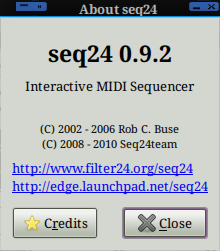
\includegraphics[scale=0.75]{menu/menu_help_about.png}
   \caption{Help About}
   \label{fig:seq24_menu_help_about}
\end{figure}

   That dialog provides access to the credits for the program, including the
   authors and the project documentor.

\begin{figure}[H]
   \centering 
   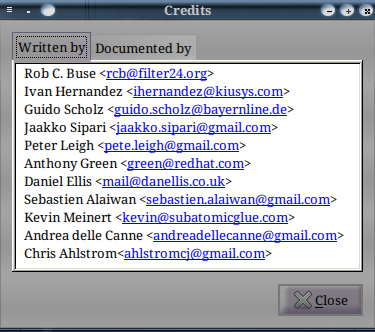
\includegraphics[scale=0.75]{menu/menu_help_credits.png}
   \caption{Help Credits}
   \label{fig:seq24_menu_help_credits}
\end{figure}

   Shows who has worked on the program, with the original author at the top
   of the list.

\begin{figure}[H]
   \centering 
   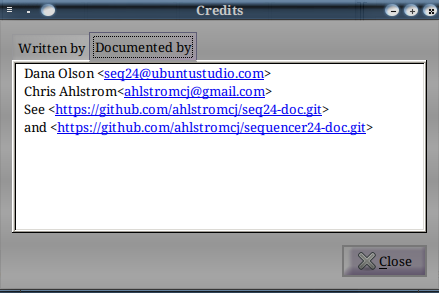
\includegraphics[scale=0.75]{menu/menu_help_doc.png}
   \caption{Help Documentation}
   \label{fig:seq24_menu_help_doc}
\end{figure}

   Shows who has documented this project.  Say, maybe "we" can get "our"
   name there someday!  \texttt{:-)}


%-------------------------------------------------------------------------------
% vim: ts=3 sw=3 et ft=tex
%-------------------------------------------------------------------------------
